\documentclass[11pt,a4paper]{article}
\usepackage[utf8]{inputenc}
\usepackage[french]{babel}
\usepackage[T1]{fontenc}

\usepackage{amsmath}
\usepackage{amsfonts}
\usepackage{amssymb}

\newcommand{\TitreMatiere}{Architecture des Ordinateurs 1}
\newcommand{\TitreSeance}{TD5 - Logique Combinatoire}
\newcommand{\SousTitreSeance}{Portes Logiques}
\newcommand{\DateCours}{Décembre 2024}
\newcommand{\AnneeScolaire}{2024-2025}
\newcommand{\Organisation}{EPITA}
\newcommand{\NomAuteurA}{Fabrice BOISSIER}
\newcommand{\MailAuteurA}{fabrice.boissier@epita.fr}
\newcommand{\NomAuteurB}{ }
\newcommand{\MailAuteurB}{ }
\newcommand{\DocKeywords}{Architecture, Logique Combinatoire, Portes Logiques ; Circuits Logiques ; Mintermes ; Maxtermes ; Tableaux de Karnaugh}
\newcommand{\DocLangue}{fr} % "en", "fr", ...

\usepackage{MetalQuickLabs}

% Babel ne traduit pas toujours bien les tableaux et autres
\renewcommand*\frenchfigurename{%
    {\scshape Figure}%
}
\renewcommand*\frenchtablename{%
    {\scshape Tableau}%
}

% Ne pas afficher le numéro de la légende sur tableaux et figures
\captionsetup{format=sanslabel}


\begin{document}

\EncadreTitre

\bigskip


%\begin{center}
%\begin{tabular}{p{5cm} p{11cm}}
%\textbf{Commandes étudiées :} & \texttt{sh}, \texttt{bash}, \texttt{man}, \texttt{ls}, \texttt{mkdir}, \texttt{touch}, \texttt{chmod}, \texttt{mv}, \texttt{rm}, \texttt{rmdir}, \texttt{cat}, \texttt{file}, \texttt{which}, \texttt{which}\\
%
%\textbf{Builtins étudiées :} & \texttt{pwd}, \texttt{cd}, \texttt{exit}, \texttt{logout}, \texttt{echo}, \texttt{umask}, \texttt{type}, \texttt{>}, \texttt{>{}>}, \texttt{<}, \texttt{<{}<}, \texttt{|}\\
%
%\textbf{Notions étudiées :} & Shell, Manuels, Fichiers, Répertoires, Droits, Redirections\\
%\end{tabular}
%\end{center}

\bigskip


Ce document a pour objectif de vous familiariser avec la logique combinatoire, c'est-à-dire les portes logiques, les formules logiques, et les méthodes permettant de réduire ces formules logiques.

\bigskip

Vous devez connaître les portes logiques et leurs tables de vérité avant de démarrer ce TD, ainsi que la loi de De Morgan impliquant la négation d'un ET ou d'un OU.

%\bigskip

%%%%%%%%%%%%%%%%%%%%%%%%%%%%%%%%%%%%%%%%%%%%%%%%

\section{Circuit logique vers formule logique}

\medskip

Transformez chaque circuit logique en formule logique.

%\medskip

\begin{center}
\begin{table}[ht!]
  \centering
  \begin{minipage}{0.50\textwidth}

\subsection*{Circuit 1}

%% Test.

\centerline{
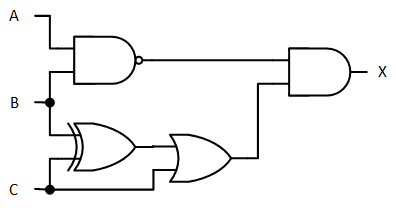
\includegraphics[scale=1.45]{./img/logique_combinatoire/circuit_logique_1.png}
}

  \end{minipage}
  \hfillx
  \begin{minipage}{0.50\textwidth}

\subsection*{Circuit 2}

%% Test.

\centerline{
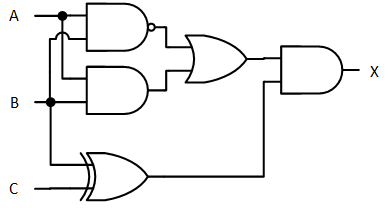
\includegraphics[scale=1.45]{./img/logique_combinatoire/circuit_logique_2.png}
}

  \end{minipage}
\end{table}
\end{center}

\vspace*{-1cm}

\subsection*{Circuit 3}

%% Test.

\centerline{
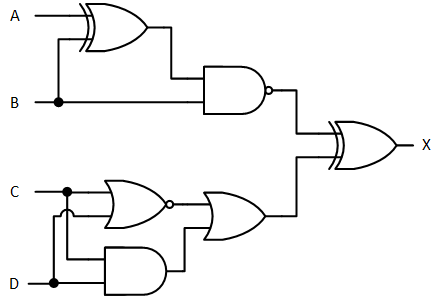
\includegraphics[scale=1.45]{./img/logique_combinatoire/circuit_logique_3.png}
}

\medskip
%%%%%%%%%%%%%%%%%%%%%%%%%

\subsection*{Circuit 4}

%% Test.

\centerline{
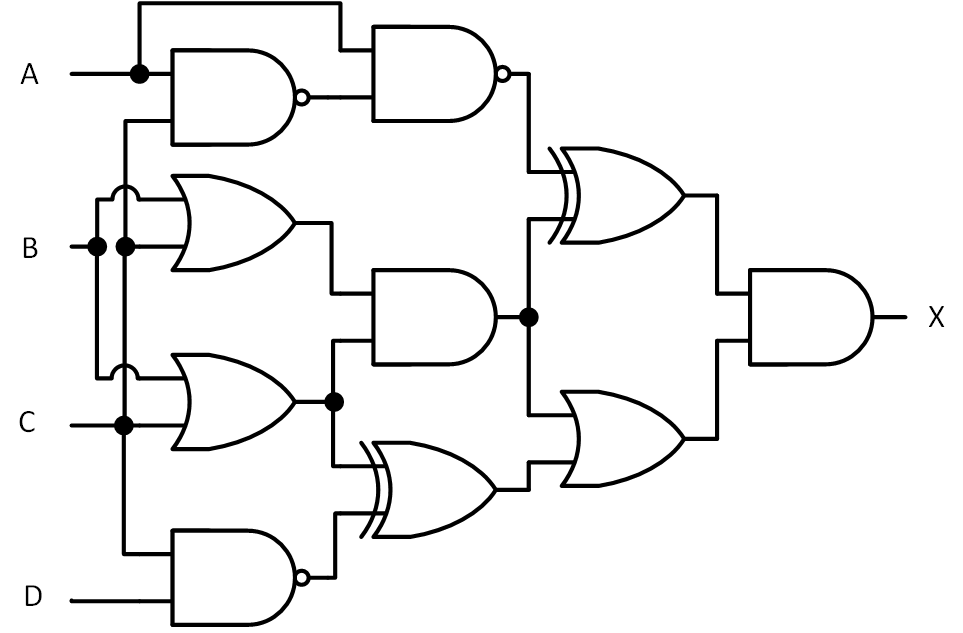
\includegraphics[scale=1.45]{./img/logique_combinatoire/circuit_logique_4.png}
}


%\bigskip
\clearpage

%%%%%%%%%%%%%%%%%%%%%%%%%%%%%%%%%%%%%%%%%%%%%%%%

\section{Portes logiques}

\medskip

Dans ces deux exercices, vous allez devoir redéfinir chaque porte logique avec l'une des deux portes fondamentales, à savoir \TTBF{NAND} et \TTBF{NOR}.

\medskip

Pour rappel voici la liste des portes logiques : \TTBF{AND}, \TTBF{OR}, \TTBF{NOT}, \TTBF{NAND}, \TTBF{NOR}, \TTBF{XOR}, \TTBF{XNOR}

\medskip

\begin{center}
\begin{table}[ht!]
  \centering
  \begin{minipage}{0.45\textwidth}

\subsection{Redéfinition à base de NAND}

Redéfinissez chaque porte logique à base de portes \TTBF{NAND}.

  \end{minipage}
  \hfillx
  \begin{minipage}{0.45\textwidth}

\subsection{Redéfinition à base de NOR}

Redéfinissez chaque porte logique à base de portes \TTBF{NOR}.

  \end{minipage}
\end{table}
\end{center}


%\bigskip

%%%%%%%%%%%%%%%%%%%%%%%%%%%%%%%%%%%%%%%%%%%%%%%%

\section{Formule logique vers circuit logique}

\medskip

Transformez ces formules logiques en circuits logiques.

\medskip

\begin{center}
\begin{table}[ht!]
  \centering
  \begin{minipage}{0.50\textwidth}

\begin{enumerate}
%  \setcounter{enumi}{0}
  \item $ ( \, (A \cdot B) \; \cdot \; \overline{(B \cdot C)} \, ) \; + \; (\overline{A} \oplus C) $
  \medskip
  \item $ (B + \overline{C}) \; \cdot \;  ( \, (B \oplus \overline{A}) \; + \; \overline{(C + A)} \, ) $
\end{enumerate}

  \end{minipage}
  \hfillx
  \begin{minipage}{0.50\textwidth}

\begin{enumerate}
  \setcounter{enumi}{2}
  \item $ ( \, (A + B) \; \oplus \; \overline{(B + C)} \, ) \; \oplus \; (C \cdot D) $
  \medskip
  \item $ (A \cdot \overline{B}) \; + \;  ( \, (B \cdot \overline{D}) \; \oplus \; (\overline{C} + D) \, ) $
\end{enumerate}

  \end{minipage}
\end{table}
\end{center}


%\bigskip

%%%%%%%%%%%%%%%%%%%%%%%%%%%%%%%%%%%%%%%%%%%%%%%%

\section{Formes canoniques et simplification}

\medskip

Pour chaque formule logique des exercices précédents, déterminez les mintermes et maxtermes de chacune d'entre elles, puis, déterminez les formules simplifiées à partir de leurs tableaux de Karnaugh associés.


\bigskip

%%%%%%%%%%%%%%%%%%%%%%%%%%%%%%%%%%%%%%%%%%%%%%%%%%%%%%%%%%%%%%%%%%%%%%%%%%%%%%%%%%%%%%%%%%%%%%%%

\bigskip

\vfillFirst

\vfillLast

\begin{center}
\textit{Ce document et ses illustrations ont été réalisés par Fabrice BOISSIER en décembre 2024}

%\textit{(dernière mise à jour octobre 2024)}
\end{center}

\end{document}
